
\index{Optics|textbf}

This section describes advanced X-ray optics
components such as mirrors and analyzer crystals.
A description of the reflectivity of a mirror is found
in section~\ref{ss:mirrorreflect}.

\section{Mulitlayer\_elliptic: The elliptic multilayer mirror}
\label{s:mirror}
\index{Optics!Mirror plane}
\component{Multilayer\_elliptic}{System}{$\theta$, $s1$, $s2$, $length$, $width$, $R$}{}{validated}
%{$R_0, Q_c, W, \alpha, reflect$}{validated}

The component {\bf Multilayer\_elliptic}
models a single rectangular reflecting multilayer mirror plate with elliptical curvature. It can be used
as a sample component, to \textit{e.g.}~assemble a Kirkpatrick-Baez focusing system 
or in combination with a double-crystal monochromator.


Figure~\ref{fig:Ellipse}\emph{Left} shows a side view of a mirror
(the blue section of the ellipse) in the McXtrace coordinate system.
At the mirror center, the mirror tangent is parallel to the $z$ axis
and the mirror normal is parallel to the $y$ axis. The width of the
mirror is $w$ and in $y-z$ plane the mirror has the curvature of an
ellipse with major axis $a$ and minor axis $b$,
%
\begin{equation} 
\frac{z^2}{ a^2} + \frac{y^2}{b^2} =1\,, \,|x| <
\frac{w}{2}\,.
\end{equation}
%
The length of the mirror is $L$. The coordinates of the mirror
center $(0,Y_0,Z_0)$ and the ellipse parameters $a$, $b$ are
determined uniquely by the central glancing angle, the source-mirror
distance and the mirror-image distance. The position of the mirror
is chosen to be at the positive side of the $y$ axis.

The input parameters of this component are:
$\theta$ [$^{\circ}$], the incident angle; 
$s1$ [m], the distance from the source to the multilayer;
$s2$ [m], the focusing distance of the multilayer;
$length$ [m], the length of the mirrors;
$width$ [m], the width of the mirror along the $x$-axis;
$R$, the reflectivity.

\subsection{Definition of the reference frames}
The direction and position of the incoming photon is defined
relative to the coordinate system illustrated in
Fig.~\ref{fig:Ellipse}\emph{Left} (in the code referred to as
\emph{McXtrace coordinate system}):
\begin{itemize}
\item the y-axis is parallel to the central mirror normal
\item the z-axis is parallel to the central mirror tangent
\item the origin is at the mirror center
\end{itemize}

However, all the calculations are conducted in another reference
frame which is illustrated in Fig.~\ref{fig:Ellipse}~\emph{Right}(in
the following referred to as the \emph{Ellipse coordinate system}):
\begin{itemize}
\item the z-axis is parallel to major axis of ellipse
\item the y-axis is parallel to minor axis of ellipse
\item the origin is at the center of the ellipse
\item the mirror center at $(0,Y_0,Z_0)$, uniquely determined by the
glancing angle at the mirror center, the source-mirror distance and
mirror-image distance.
\end{itemize}

\begin{figure}[htb!]
\centering
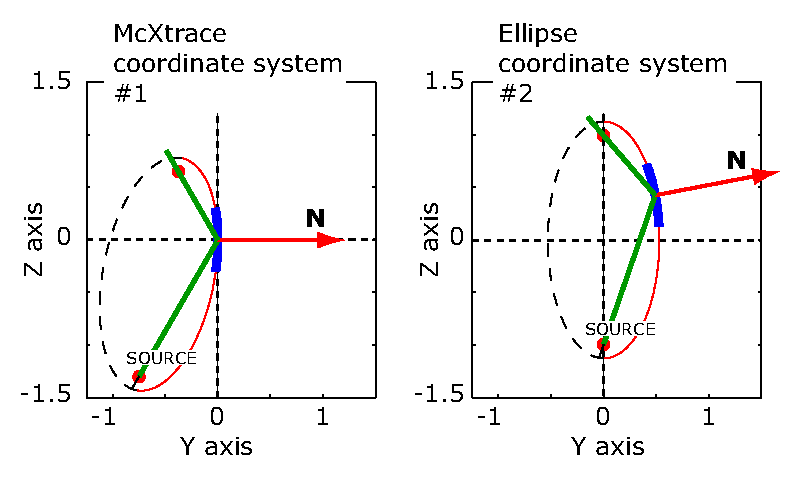
\includegraphics[width=0.95\linewidth]{figures/ellipse.eps}
 \caption{The same image in different coordinate systems.\newline \emph{Left}:
 \emph{McXtrace System} with the y-axis is parallel to the central mirror normal, the z-axis
 is parallel to the central mirror tangent and the origin is at the mirror
 center. \newline
 \emph{Right}: \emph{Ellipse System} with
the z-axis parallel to major axis of ellipse, the y-axis is parallel
to minor axis of ellipse and the origin is at the center of the
ellipse. }\label{fig:Ellipse}
\end{figure}


\subsection{Algorithm}
\begin{enumerate}
\item The photon is generated with a starting point $\bf{S}$ and a direction
$\bf{V}_\textrm{in}$ defined in the \emph{McXtrace} coordinate
system.
\item All calculations are performed in the \emph{Ellipse} coordinate system,
so to proceed the basis is changed to that reference frame.
\item The 2 intersections of the ray with the ellipse are determined.
\item It is checked if any of the intersections are within the area
defined by the mirror.
\item If one of the solutions is valid, the reflection of that ray is
determined.
\item The coordinates of the starting point and direction of the
reflected ray are calculated using the basis of the \emph{McXtrace}
coordinate system.
\end{enumerate}


\section{Reflection of the ray in the mirror}
\begin{figure}[htb!]
\centering
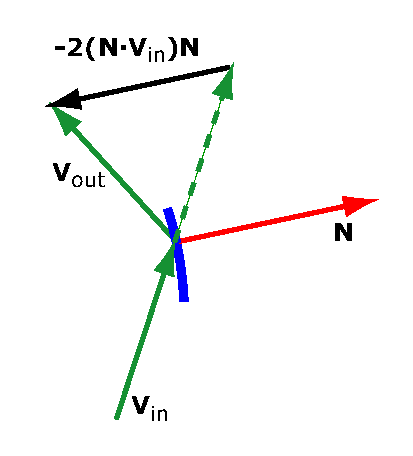
\includegraphics[width=0.3\linewidth]{figures/Dotproduct.eps}
 \caption{The reflection of the unit vector $\bf{V}_\textrm{in}$ in the mirror with the normal unit
 vector ${\bf{N}}$ is ${\bf{V}}_\textrm{out} = {\bf{V}}_\textrm{in} -2({\bf{N}}\cdot{\bf{V}}_\textrm{in}){\bf{N}}$}\label{fig:dotProduct}
\end{figure}

The tangent and normal to the ellipse $z^2/a^2 + y^2/b^2=1$ at the
point $(Y,Z)$ are found by implicit differentiation: \begin{equation} 
\frac{2z}{a^2} + \frac{2y}{b^2} \,\frac{dy}{dz} = 0\,, \end{equation} so at the
point $(Y,Z)$ the slope of the tangent is $\frac{dy}{dz} =
-\frac{Z\,b^2}{Y\,a^2}$. The slope of the normal is minus the
inverse of the tangent slope, so the coordinates of the mirror
normal are \begin{equation} N_x = 0 \quad N_y = \frac{a^2\,Y}{b^2\,Z} \quad N_z =
1\,. \end{equation} With $\bf{V}_\textrm{in}$ and $\bf{N}$ denoting unit
vectors (direction and normal respectively), the direction of the
reflected ray is calculated as \begin{equation} {\bf{V}}_\textrm{out} =
{\bf{V}}_\textrm{in} -2({\bf{N}}\cdot{\bf{V}}_\textrm{in}){\bf{N}} =
        \left(
      \begin{array}{c}
        V_{\textrm{in}x} - 2({\bf{N}}\cdot{\bf{V}}_\textrm{in})N_x \\
               V_{\textrm{in}y} - 2({\bf{N}}\cdot{\bf{V}}_\textrm{in})N_y \\
                V_{\textrm{in}z} - 2({\bf{N}}\cdot{\bf{V}}_\textrm{in})N_z \\
      \end{array}
    \right)
\end{equation}


\subsection{Mirror reflectivity}
\label{ss:mirrorreflecttable}

At present, the Multilayer\_elliptic Mirror component uses a reflectivity table $reflect$, 
which 1st column is q [$\AA^{-1}$] and from the 2nd column on as the reflectivity $R$ in [0-1]
as function of tabulated energy [$KeV$]. 
An example file, calculated for a particular $Si/W$ multilayer, is provided (\verb+reflectivity.txt+).
User provided reflectivity data files can be parsed by the component.



\section{Mirror\_curved}
\label{mirror-curved}
\index{Mirror!Cylindrically curved mirror}
\component{Mirror\_curved}{System}{\textit{radius,length,width}}{\textit{coating,R0}}{}
 
Models a cylindrical mirror, positioned in the XZ-plane curving towards
positive X. The input parameter \textit{radius} defines the radius of curvature
and the mirror size is given by \textit{length} and \textit{width} where length
and width is along Z and Y respectively. $coating$ and $R0$ are mutually
exclusive. If \textit{R0} is nonzero, it is taken as the reflectivity value,
irrespective of wavelength, whereas coating nominates a file from which to read
values for $f_1$ and $f_2$. See~\cite{NIST-ffast} for definitions. For
elements $Z\in[1,92]$ datafiles are distributed with the McXtrace system that
may be used as: \verb+coating="Rh.txt"+. or \verb+coating="Al.txt"+. 
